\chapter{Resultados e Discussão}

\subsection{Rede de Sensores Sem Fio}
Nesta seção serão apresentados os resultados parciais obtidos no desenvolvimento da Rede de Sensores sem fio.

\subsubsection{Testes utilizando a IDE Arduino}
Inicialmente foram efetuados testes utilizando o módulo NodeMCU sendo programado utilizando-se a IDE do Arduino. Para efetuar a leitura do sensor de temperatura e umidade do ar de uma forma mais simples foi utilizado a biblioteca DHT.h. Como resultado foram obtidos os seguintes códigos:

\begin{table}[H]
\centering
\caption{Função que lê a temperatura do sensor}
\vspace{-\baselineskip}
\begin{minted}[
frame=single,
framesep=2mm,
baselinestretch=1.2,
bgcolor=LightGray,
fontsize=\footnotesize,
% linenos
]{c++}

float getTemperature() {
    float temp = dht.readTemperature();
    
    if (isnan(temp)) {
        Serial.println("Failed to read from DHT sensor!");
        return;
    }
    
    return temp;
}
\end{minted}
\vspace{-1.2cm}
\label{tab:funcao-temperatura}
\fonte{Do autor}
\end{table}

O trecho de código \ref{tab:funcao-temperatura} é responsável por efetuar a coleta de temperatura pelo sensor DHT11, essa temperatura pode ser coletada em Celsius ou em Fahrenheit, neste caso iremos utilizar apenas o valor em celsius.

\begin{table}[H]
\centering
\caption{Função que lê a umidade do sensor}
\vspace{-\baselineskip}
\begin{minted}[
frame=single,
framesep=2mm,
baselinestretch=1.2,
bgcolor=LightGray,
fontsize=\footnotesize,
% linenos
]{c++}

float getHumidity() {
    float hum = dht.readHumidity();
    
    if (isnan(hum)) {
        Serial.println("Failed to read from DHT sensor!");
        return;
    }
    
    return hum;
}
\end{minted}
\vspace{-1.2cm}
\label{tab:funcao-umidade}
\fonte{Do autor}
\end{table}

O trecho de código \ref{tab:funcao-umidade} é responsável por efetuar a coleta de umidade do ar pelo sensor DHT11. O valor é coletado em porcentagem.

\begin{table}[H]
\centering
\caption{Função que envia um objeto JSON com os valores medidos}
\vspace{-\baselineskip}
\begin{minted}[
frame=single,
framesep=2mm,
baselinestretch=1.2,
bgcolor=LightGray,
fontsize=\footnotesize,
% linenos
]{c++}

void sendRequest(WiFiClient client) {
  StaticJsonBuffer<400> jsonBuffer;

  JsonObject& data = jsonBuffer.createObject();

  data["humidity"] = getHumidity();
  data["temperature"] = getTemperature();

  client.println(String("POST ") + url + " HTTP/1.1");
  client.println(String("Host: ") + host);
  client.println("Cache-Control: no-cache");
  client.println("Content-Type: application/json");
  client.print("Content-Length: ");
  client.println(data.measurePrettyLength());

  client.println();

  data.prettyPrintTo(client);
}
\end{minted}
\vspace{-1.2cm}
\label{tab:funcao-request}
\fonte{Do autor}
\end{table}

Esta função (algoritmo \ref{tab:funcao-request}) monta um objeto JSON contendo os valores obtidos pelo sensor de temperatura e umidade do ar DHT11. Após montar este objeto é feito uma requisição do tipo POST na aplicação Web onde será armazenado em um banco de dados.

\subsubsection{Desenvolvimento utilizando MicroPython}

Depois de realizados estes testes utilizando a IDE do Arduino, foi instalado o \textit{firmware} MicroPython que possibilita que o módulo NodeMCU seja programado utilizando-se a linguagem de Programação Python.

A programação foi realizada da seguinte forma, o nó se conecta a uma rede \textit{wifi} (algoritmo \ref{tab:funcao-conecta}) e, após estar conectado, faz a coleta de dados de todos os sensores ligados a ele (algoritmo \ref{tab:funcao-coleta}). Após coletar os dados, eles são publicados no broker mqtt (algoritmo \ref{tab:funcao-publica}), feito isso, o nó entra em modo \textit{sleep}. Este ciclo irá se repetir constantemente, sendo que o nó será acordado apos um intervalo de tempo pré definido.

\begin{table}[H]
\centering
\caption{Função que conecta o nó a uma rede wifi}
\vspace{-\baselineskip}
\begin{minted}[
frame=single,
framesep=2mm,
baselinestretch=1.2,
bgcolor=LightGray,
fontsize=\footnotesize,
% linenos
]{python}

def do_connect(self):
    SSID = self.conf['network']['ssid']
    PASSWORD = self.conf['network']['password']

    self.wlan = network.WLAN(network.STA_IF)
    self.wlan.active(True)
    if not self.wlan.isconnected():
        self.wlan.connect(SSID, PASSWORD)

        while not self.wlan.isconnected():
            pass

\end{minted}
\vspace{-1.2cm}
\label{tab:funcao-conecta}
\fonte{Do autor}
\end{table}

\begin{table}[H]
\centering
\caption{Função que coleta os dados dos sensores}
\vspace{-\baselineskip}
\begin{minted}[
frame=single,
framesep=2mm,
baselinestretch=1.2,
bgcolor=LightGray,
fontsize=\footnotesize,
% linenos
]{python}

def get_sensors_data(self):
    dht_pin = self.conf['sensors']['dht11']

    humidity = Humidity(dht_pin)
    temperature = Temperature(dht_pin)

    data = {
        'humidity': humidity.get_humidity(),
        'temperature': temperature.get_temperature()
    }

    return data

\end{minted}
\vspace{-1.2cm}
\label{tab:funcao-coleta}
\fonte{Do autor}
\end{table}

\begin{table}[H]
\centering
\caption{Função que publica os dados}
\vspace{-\baselineskip}
\begin{minted}[
frame=single,
framesep=2mm,
baselinestretch=1.2,
bgcolor=LightGray,
fontsize=\footnotesize,
% linenos
]{python}

def send_data(self):
    data = self.mount_request_body()
    data = json.dumps(data)
    
    topic = self.conf['mqtt']['topic']

    self.mqtt_client.publish(topic, data)

\end{minted}
\vspace{-1.2cm}
\label{tab:funcao-publica}
\fonte{Do autor}
\end{table}

\subsection{Aplicação Web}
Nesta seção serão apresentados os resultados parciais obtidos quanto ao desenvolvimento da aplicação web, seguindo os passos listados na Metodologia, seção 4.

\subsubsection{Levantamento e Análise de Requisitos}
Foram levantados os requisitos que atendem às necessidades do setor. Feito este levantamento, foi definido um escopo para se dar inicio ao desenvolvimento, foi definido que as funcionalidades a serem implementadas serão: 

\begin{itemize}[itemsep=0em]
\item Manter usuários
\item Manter experimentos
\item Manter medições
\item Consultar relatórios
\end{itemize}

\subsubsection{Projeto de \textit{software}}
A figura \ref{fig:caso-de-uso} mostra o diagrama de caso de uso elaborados de acordo com os requisitos levantados na etapa anterior.

\subsubsection{Implementação}
A figura \ref{fig:tela-login} mostra a tela de autenticação, que é necessário ser efetuado para que o usuário tenha acesso às funcionalidades do sistema. A figura \ref{fig:tela-dashboard} mostra o \textit{dashboard} do sistema, nele são listados as medições realizadas nos últimos 60 minutos. À medida que as medições são salvas no banco de dados os gráficos do \textit{dashboard} são atualizados.

\begin{figure}[H]
    \centering
    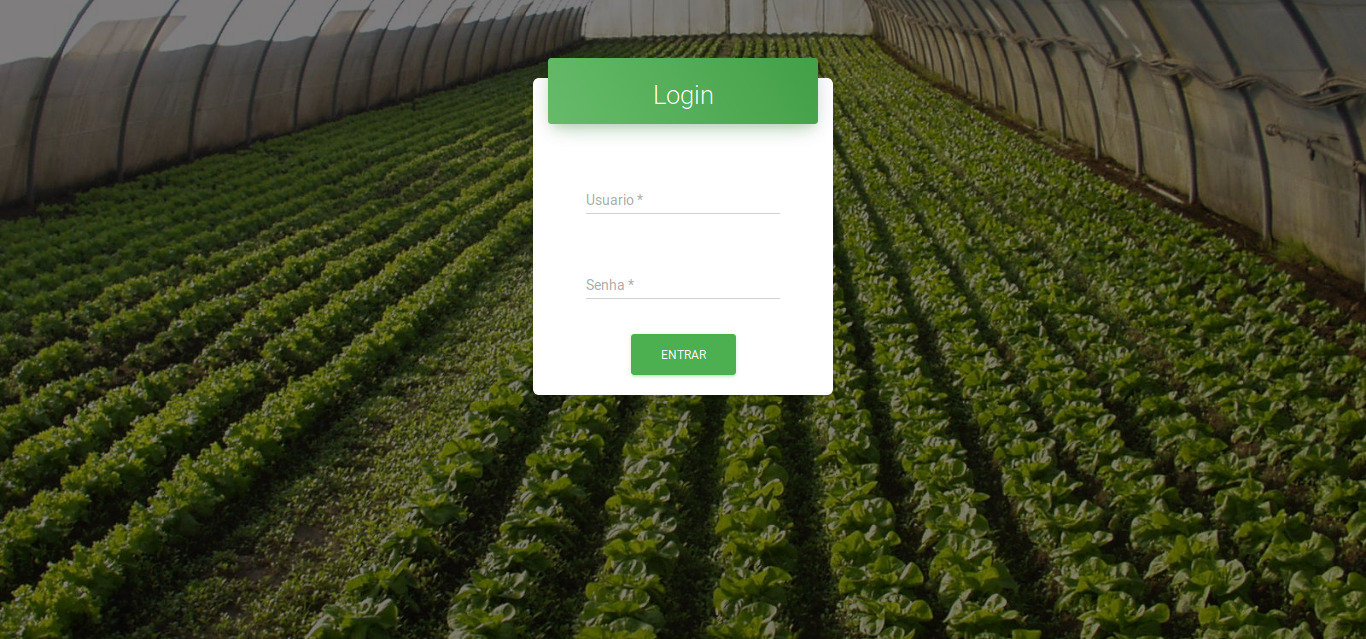
\includegraphics[scale=0.3]{04-figuras/tela_login.jpg}
    \caption{Tela de \textit{login} do sistema}
    \vspace{-\baselineskip}
    \fonte{Do autor}
    \label{fig:tela-login}
\end{figure}

\begin{figure}[H]
    \centering
    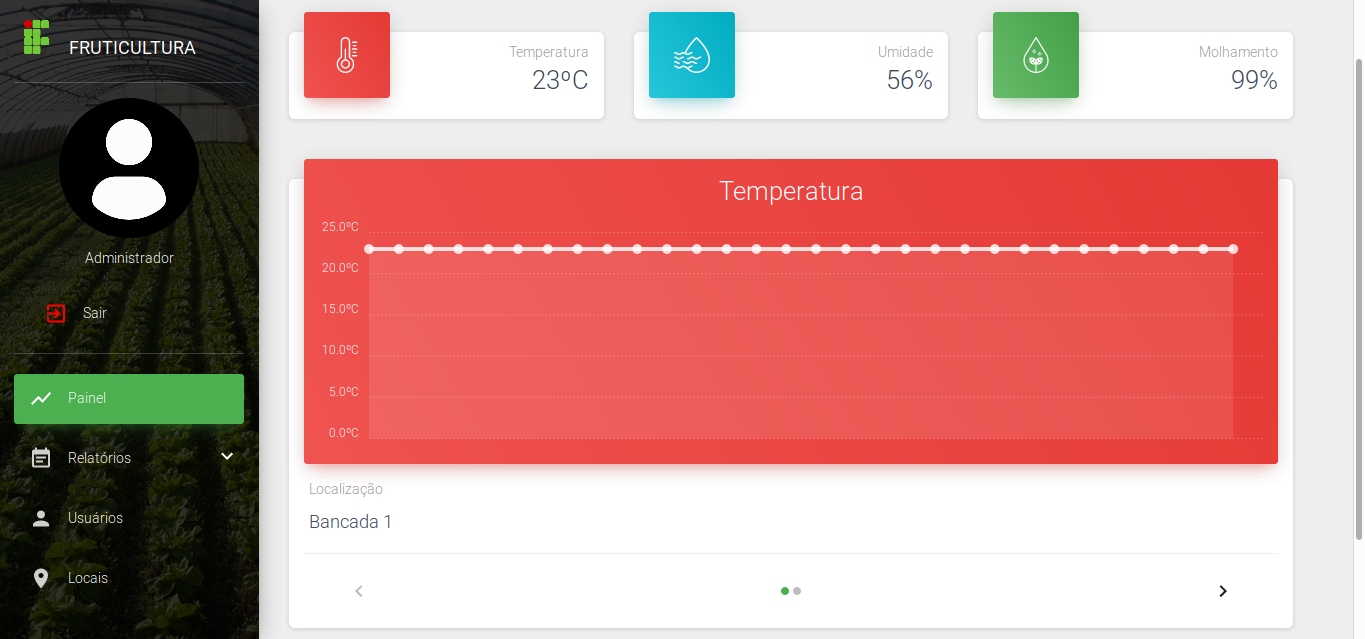
\includegraphics[scale=0.3]{04-figuras/tela_painel.png}
    \caption{Painel do sistema}
    \vspace{-\baselineskip}
    \fonte{Do autor}
    \label{fig:tela-dashboard}
\end{figure}

A figura \ref{fig:tela-listar-usuarios} mostra a tela onde é possível fazer a listagem dos usuários cadastrados no sistema, tendo também as ações de cadastrar ou excluir algum usuário listado. Já na figura \ref{fig:tela-cadastrar-usuario} temos o formulário utilizado para cadastrar um novo usuário e também atualizar as informações de um usuário já existente.

\begin{figure}[H]
    \centering
    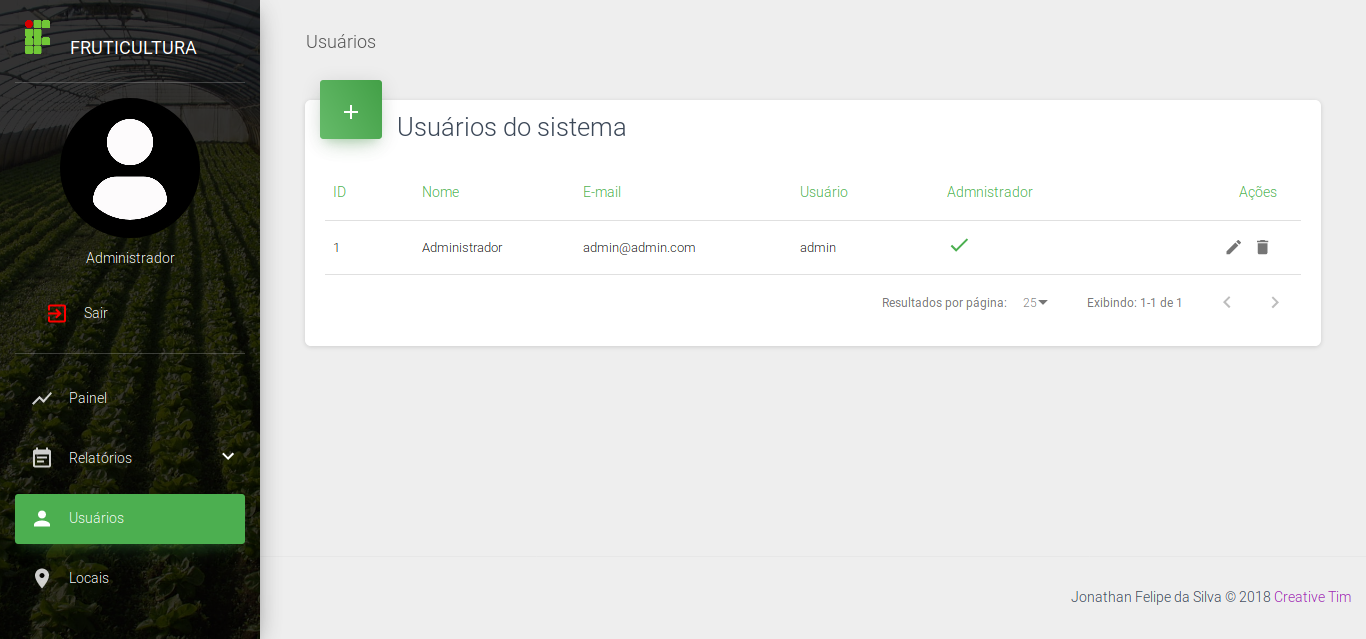
\includegraphics[scale=0.3]{04-figuras/tela_listar_usuarios.png}
    \caption{Tela de listar usuários}
    \vspace{-\baselineskip}
    \fonte{Do autor}
    \label{fig:tela-listar-usuarios}
\end{figure}

\begin{figure}[H]
    \centering
    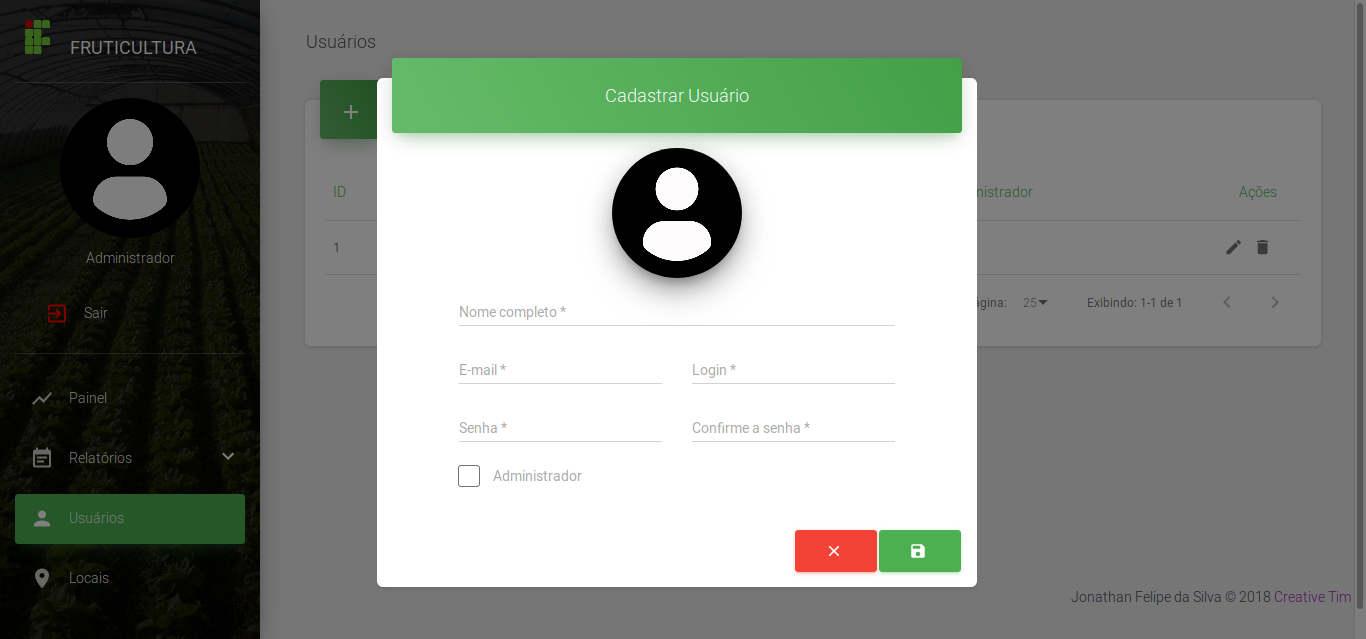
\includegraphics[scale=0.3]{04-figuras/tela_cadastrar_usuario.png}
    \caption{Tela de cadastrar novo usuário}
    \vspace{-\baselineskip}
    \fonte{Do autor}
    \label{fig:tela-cadastrar-usuario}
\end{figure}

A figura \ref{fig:tela-listar-locais} mostra a tela onde é possível fazer a listagem dos locais já cadastrados no sistema, tendo também as ações de cadastrar ou excluir algum local listado. Já na figura \ref{fig:tela-cadastrar-usuario} temos o formulário utilizado para cadastrar um novo local e também atualizar as informações de um local já cadastrado.

\begin{figure}[H]
    \centering
    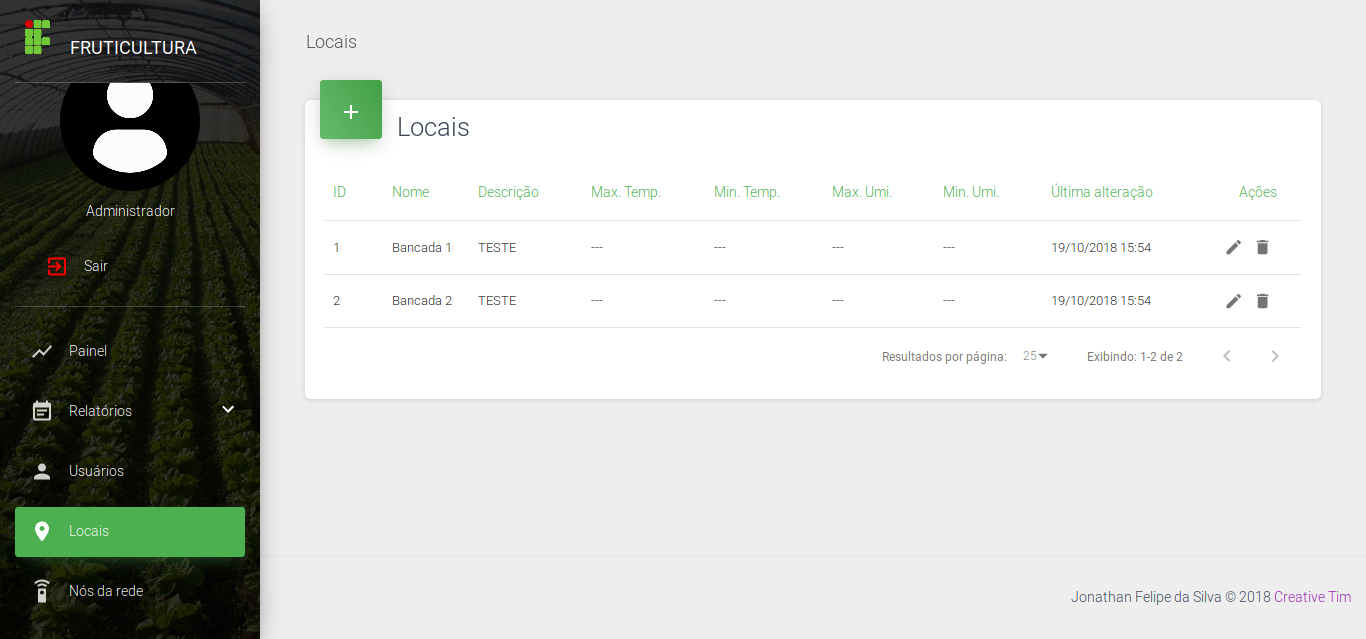
\includegraphics[scale=0.3]{04-figuras/tela_lista_locais.png}
    \caption{Tela de listar localizações dos nós}
    \vspace{-\baselineskip}
    \fonte{Do autor}
    \label{fig:tela-listar-locais}
\end{figure}

\begin{figure}[H]
    \centering
    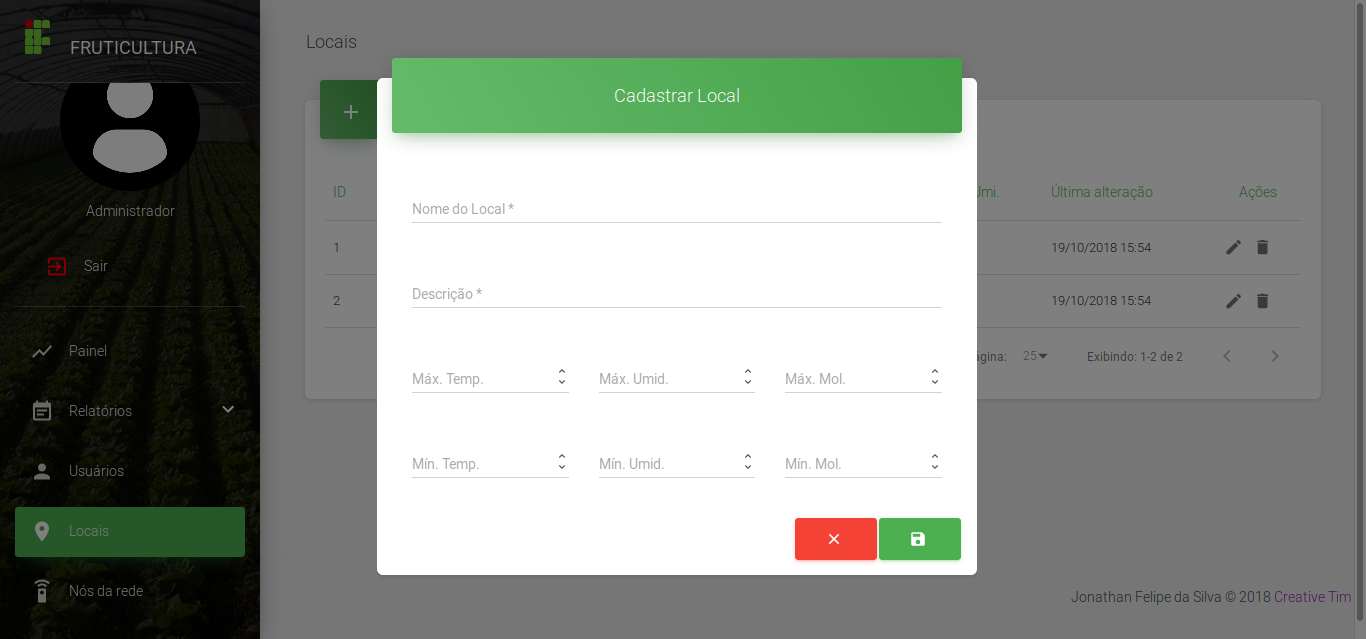
\includegraphics[scale=0.3]{04-figuras/tela_cadastra_local.png}
    \caption{Tela de cadastrar novo local}
    \vspace{-\baselineskip}
    \fonte{Do autor}
    \label{fig:tela-cadastrar-local}
\end{figure}

A figura \ref{fig:tela-listar-nos} mostra a tela onde é possível fazer a listagem dos nós já cadastrados no sistema, tendo também as ações de cadastrar ou excluir algum nó listado. Já na figura \ref{fig:tela-cadastrar-no} temos o formulário utilizado para cadastrar um novo nó e também atualizar as informações de um nó já cadastrado.

\begin{figure}[H]
    \centering
    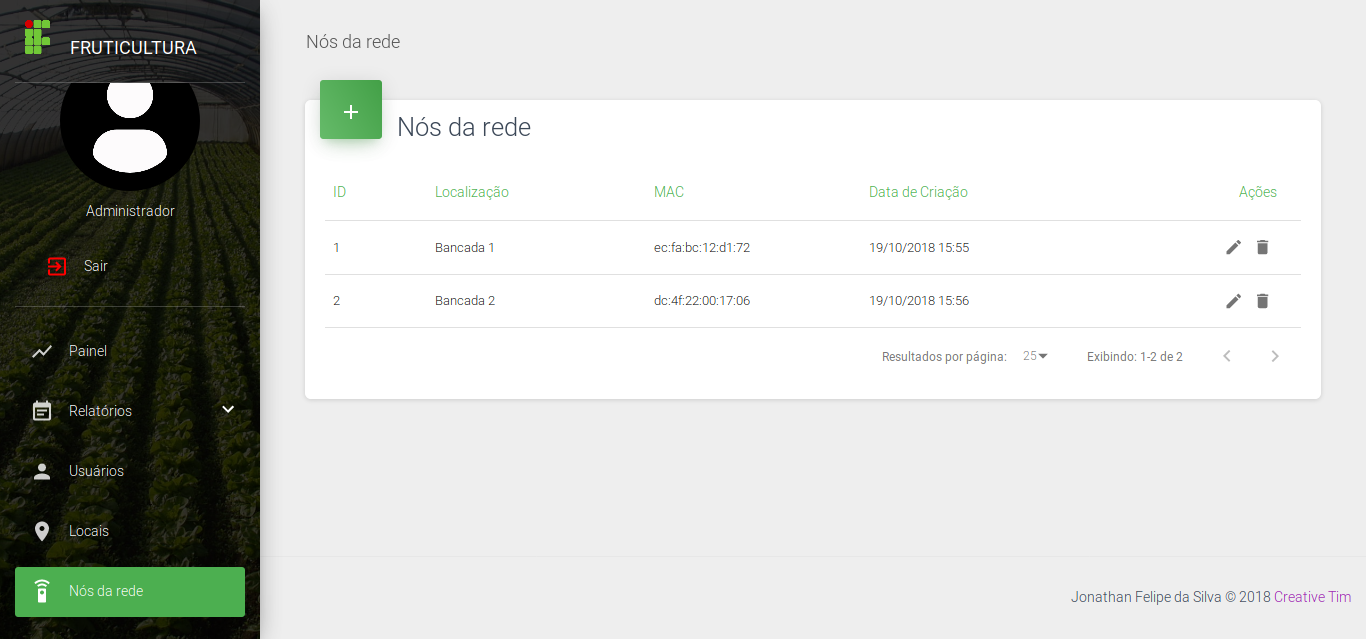
\includegraphics[scale=0.3]{04-figuras/tela_lista_no.png}
    \caption{Tela de listar nós da rede}
    \vspace{-\baselineskip}
    \fonte{Do autor}
    \label{fig:tela-listar-nos}
\end{figure}

\begin{figure}[H]
    \centering
    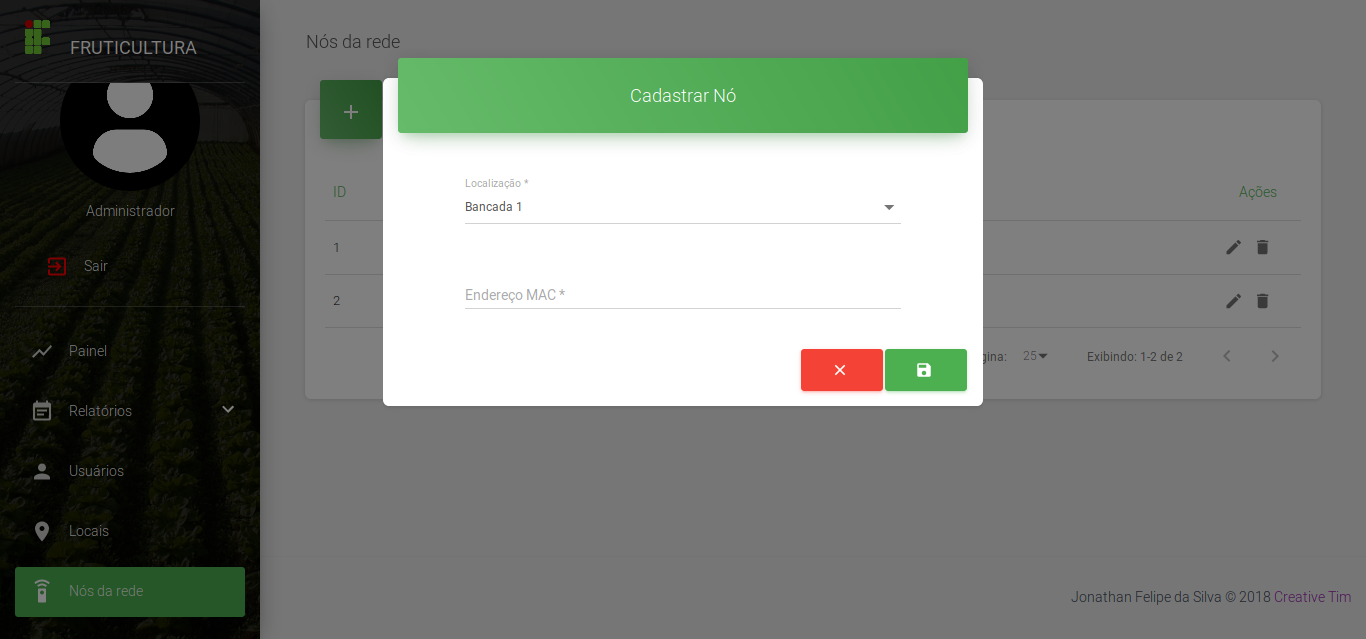
\includegraphics[scale=0.3]{04-figuras/tela_cadastra_no.png}
    \caption{Tela de cadastrar novo nó}
    \vspace{-\baselineskip}
    \fonte{Do autor}
    \label{fig:tela-cadastrar-no}
\end{figure}


A figura \ref{fig:tela-relatorio-medicoes} mostra a tela onde é emitir um relatório das medições realizadas pela rede em um determinado intervalo de tempo, além de também ter como ação visualizar todas as medições do dia. Já na figura \ref{fig:tela-relatorio-medicoes-dia} temos a listagem de todas as medições realizadas no dia em questão.

\begin{figure}[H]
    \centering
    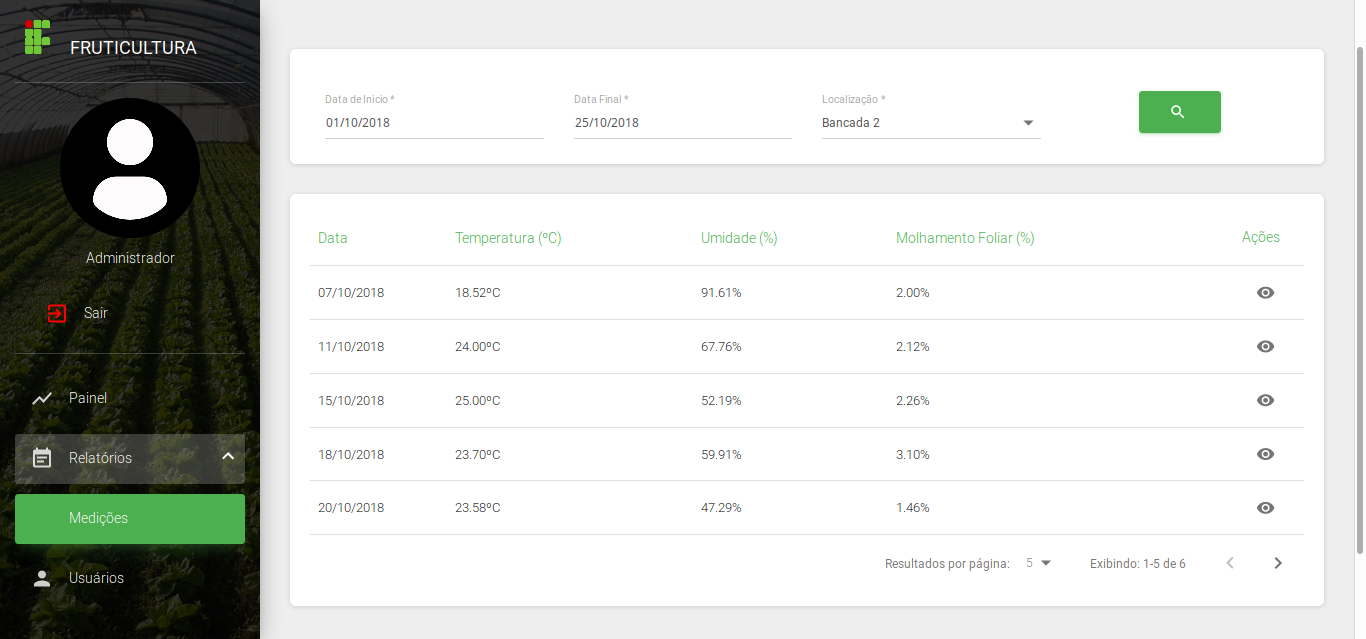
\includegraphics[scale=0.3]{04-figuras/tela_relatorio_medicoes.png}
    \caption{Tela de medições de um intervalo.}
    \vspace{-\baselineskip}
    \fonte{Do autor}
    \label{fig:tela-relatorio-medicoes}
\end{figure}

\begin{figure}[H]
    \centering
    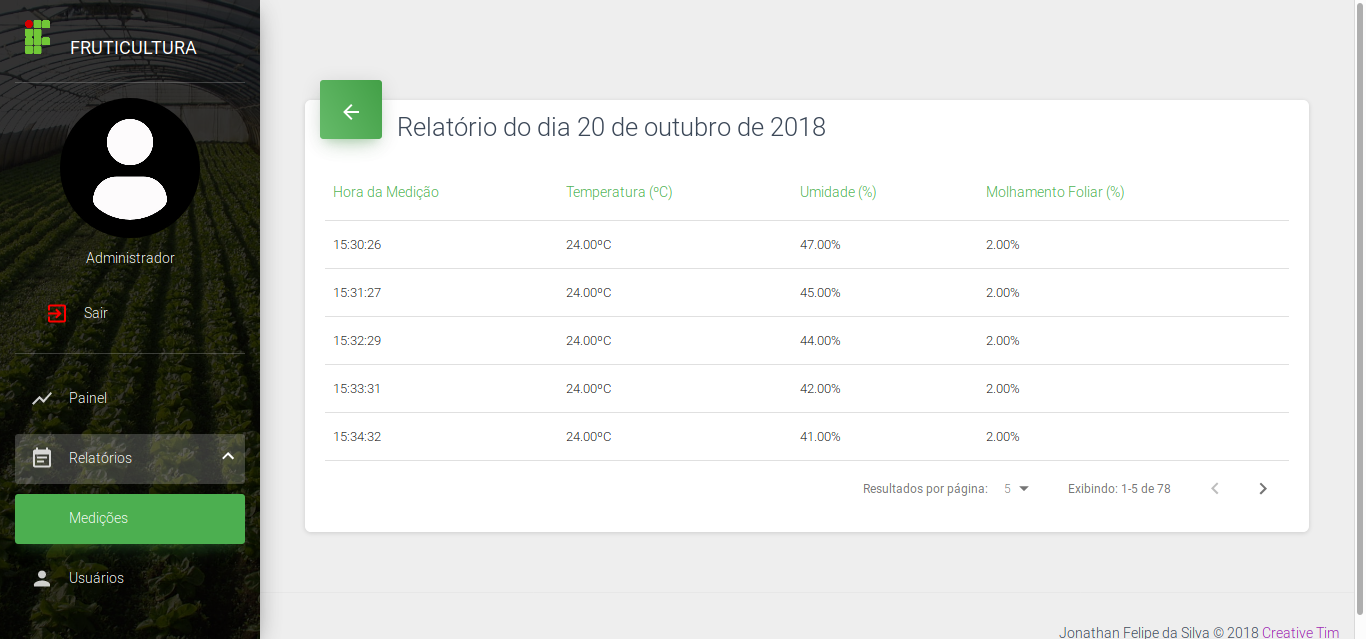
\includegraphics[scale=0.3]{04-figuras/tela_relatorio_medicoes_dia.png}
    \caption{Tela de medições de um dia.}
    \vspace{-\baselineskip}
    \fonte{Do autor}
    \label{fig:tela-relatorio-medicoes-dia}
\end{figure}

\subsection{Configuração de um servidor}
Para se dar inicio aos testes do trabalho era necessário um servidor tanto para a aplicação web quanto para o \textit{broker} mqtt. Diante essa demanda foi criado uma conta na Amazon Web Services (AWS)\footnote{Fonte: \url{https://aws.amazon.com/pt/}}, que é uma plataforma de serviços de computação em nuvem.

Com uma maquina virtual Linux disponibilizada pela AWS foi possível fazer a configuração de um servidor web com o Nginx\footnote{Fonte: \url{https://www.nginx.com/}}
e também a configuração do \textit{broker} mqtt Mosquitto.

Após concluir as configurações foi realizado o \textit{deploy} da aplicação, tanto backend quanto frontend, para o servidor\footnote{A aplicação pode ser acessada em: \url{http://18.231.25.86}}.